\documentclass{article}

%%%%
% PLOTS mapas y conglomerados
% bibliografia
%%%%
\usepackage[T1]{fontenc} %%%
\usepackage[utf8]{inputenc}
\usepackage{longtable}
\usepackage{authblk}
\usepackage{adjustbox}



\usepackage{natbib}

\title{LOS \'INDICES DE COLOMBIA}
% autores
\renewcommand\Authand{, y }
\author[1]{\normalsize Santiago Serrano}


\affil[1,2]{\small  Escuela de Ingenier\'ia,Universidad de los Andes\\
\texttt{{s.serrano11}@uniandes.edu.col}}
\affil[1]{\small Instituto de altas investigaciones financieras\\
Banco del Parque\\
\texttt{delcurso@bp.com.col}}

\date{05 de Julio de 2018}

%%%%
\usepackage{Sweave}
\begin{document}
\Sconcordance{concordance:FinaldeR3.tex:FinaldeR3.Rnw:%
1 29 1 1 0 25 1 1 13 4 1 1 6 15 0 1 3 11 1 1 10 1 2 9 1 1 17 1 6 15 1 1 %
4 12 0 1 3 3 1 1 14 13 0 1 2 6 1 1 4 1 3 13 1 1 6 1 4 31 0 1 2 10 1 1 %
75 8 1 1 17 1 3 11 1}


\maketitle



\begin{abstract}
El proposito principal de este trabajo es describir los procesos para partir una poblacion N-dimensional en partes de k tamano en forma de una muestra. El proceso, que se denomina 'k-means' aparece para dar particiones que son rasonablemente eficientes en el sentido de las variables dentro de las categorias. Eso es, que si p es la probabilidad de densidad para la poblacion S, S=s1,s2,...,Sn. La parte de En y de ui siendo i=1,2,3,..,k es el promedio condicional de p sobre S. Diremos de ahora en adelante en el documento 'tiende a ser bajo' para referirnos en principio a las consideraciones intuitivas y corroboradas del analisis matematico y practicas computacionales.
\end{abstract}

\section*{Introducci\'on}

The main purpose of this paper is to descrube a procces for partitioning an N-dimensional population into k sets on the basis of a sample. Th procvess, which is called 'k-means', appears to five partitions which are reasonably effcient in the sense of within-class variance. That is, if p is the probability mass functon for the population, S= S1,S2,..,Sn is a partition of En. We say 'tends to be low' primarily because of intutive considerations, corroborated to some extent by mthematical analysis and practical computational experience.


Comencemos viendo que hay en la secci\'on \ref{univariada} en la p\'agina \pageref{univariada}.

\clearpage



\section{Exploraci\'on Univariada}\label{univariada}

En esta secci\'on exploro cada \'indice. En esta secci\'on exploro cada \'indice. En esta secci\'on exploro cada \'indice. En esta secci\'on exploro cada \'indice. En esta secci\'on exploro cada \'indice. En esta secci\'on exploro cada \'indice. En esta secci\'on exploro cada \'indice. En esta secci\'`n exploro cada \'indice. En esta secci\'on exploro cada \'indice.


Para conocer el comportamiento de las variables se ha preparado  donde se describe la distribuci\'on de las modalidades de cada variable. Los n\'umeros representan la situaci\'on de algun pa\'is en ese indicador, donde el mayor valor num\'erico es la mejor situaci\'on.



% Table created by stargazer v.5.2.2 by Marek Hlavac, Harvard University. E-mail: hlavac at fas.harvard.edu
% Date and time: Thu, Jul 05, 2018 - 16:16:14
\begin{table}[!htbp] \centering 
  \caption{Medidas estad<U+00ED>sticas} 
  \label{stats} 
\begin{tabular}{@{\extracolsep{5pt}}lccccc} 
\\[-1.8ex]\hline 
\hline \\[-1.8ex] 
Statistic & \multicolumn{1}{c}{Mean} & \multicolumn{1}{c}{St. Dev.} & \multicolumn{1}{c}{Max} & \multicolumn{1}{c}{Min} & \multicolumn{1}{c}{Median} \\ 
\hline \\[-1.8ex] 
IDH & 0.802 & 0.042 & 0.879 & 0.691 & 0.804 \\ 
Poblaci..n.Cabecera & 1,196,730.000 & 1,982,287.000 & 10,070,801 & 13,090 & 717,197 \\ 
Poblaci..n.Resto & 360,590.300 & 331,887.600 & 1,428,858 & 21,926 & 268,111.5 \\ 
Poblaci..n.Total & 1,557,320.000 & 2,202,522.000 & 10,985,285 & 43,446 & 1,028,429 \\ 
\hline \\[-1.8ex] 
\end{tabular} 
\end{table} 
Como apreciamos en  los pa\'ises en la mejor situaci\'on son los menos, salvo en el caso del \emph{\'indice de libertas mundial}\footnote{N\'otese que esto se puede deber a la {\bf menor} cantidad de categor\'ias.}

\clearpage

Para resaltar lo anterior, tenemos la Figura \ref{barplots} en la p\'agina \pageref{barplots}. 


%%%%% figure
\begin{figure}[h]
\centering

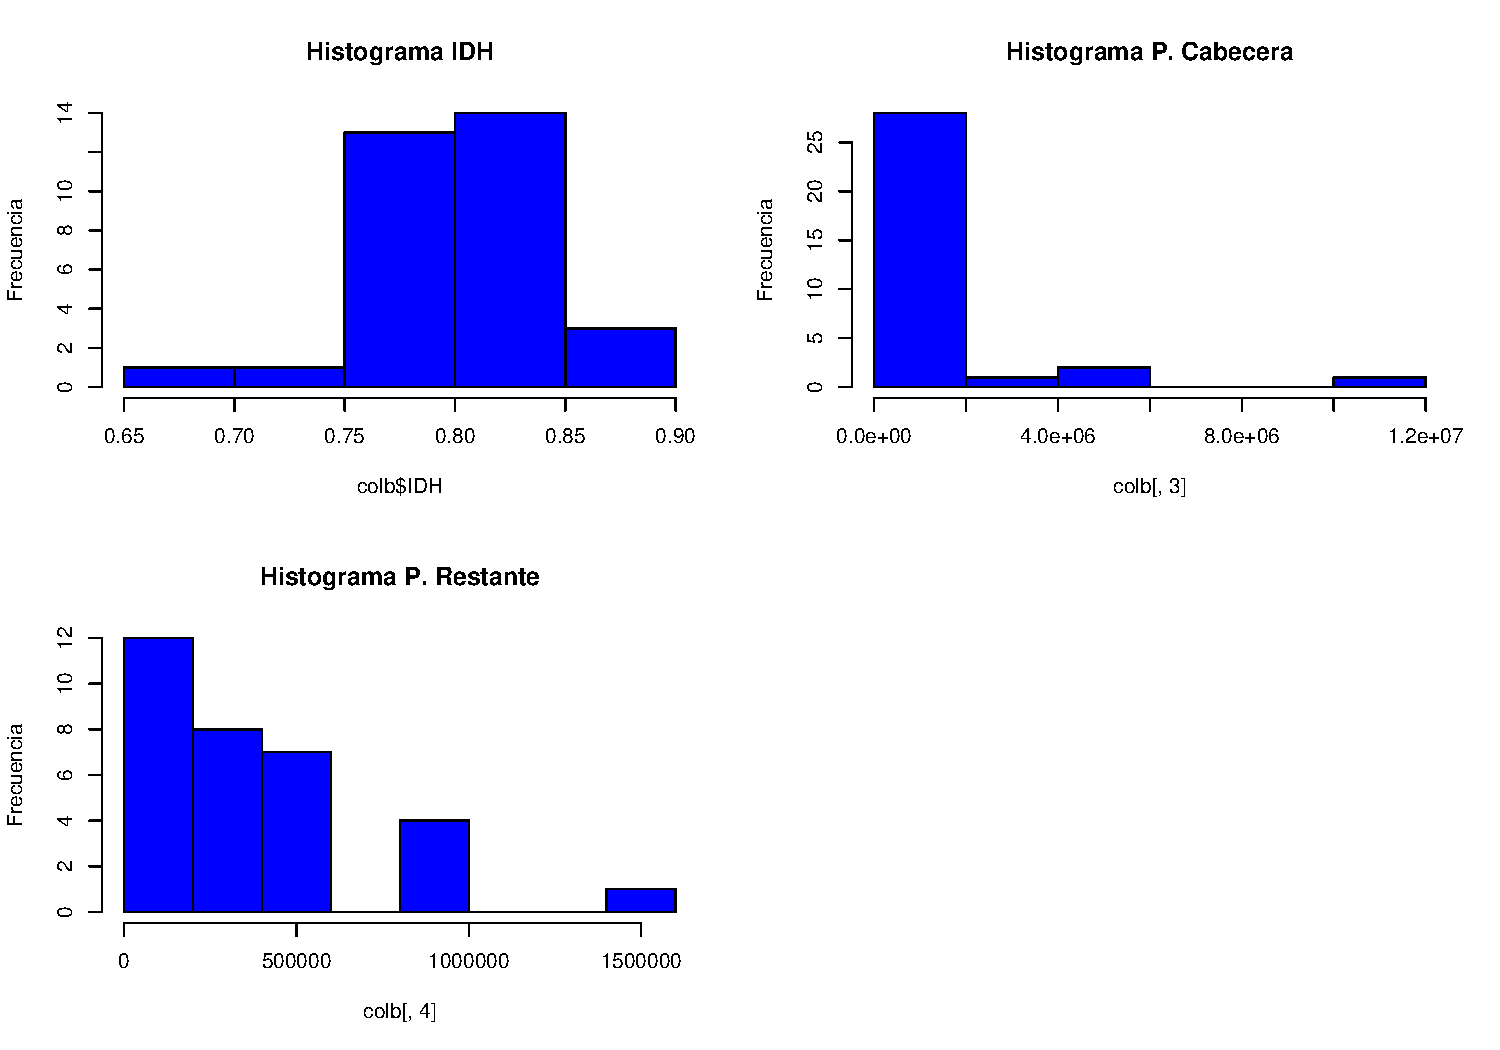
\includegraphics{FinaldeR3-hist}



\caption{Distribuci\'on de Indicadores}
\label{barplots}
\end{figure}

Adem\'as de la distribuci\'on de los variable, es importante saber el valor central. Como los valores son de naturaleza ordinal debemos pedir la {\bf mediana} y otras medidas de posici\'on (como los \emph{cuartiles}, los que no pediremos pues son pocos valores). La mediana de cada variable la mostramos enn la p\'agina.


#<<log, echo=FALSE,fig=TRUE>>=

# dado el sesgo de las pobaciones, 
# podriamos transformarla para que se acerque a la 
# normalidad
#par(mfrow=c(2,2))
###
colb$cabeLog=log(colb[,3])
colb$restoLog=log(colb[,4])


hist(log(colb$poblacion.cabecera),main="Logaritmo de la poblacion",ylab="Frecuencia", col="RED")
###
hist(colb$cabeLog,main="Logaritomo de la poblacion cabecera",ylab="Frecuencia",col="RED")
###
hist(colb$restoLog,main="Logaritmo de la poblacion resto",ylab="Frecuencia",col="RED")
###

#hist(colb$cabeLog)
#hist(colb$restoLog)


#<<summary, fig=TRUE, echo=false>>==
# dado el sesgo de las pobaciones, 
# podriamos transformarla para que se acerque a la 
# normalidad

par(mfrow=c(2,2))

colb$cabeLog=log(colb$poblacion.cabecera)
colb$restoLog=log(colb$poblacion.resto)

title='Logaritmo de la poblaci<U+00F3>n de cabecera'
paleta='red'
demoTableRelPlot=hist(colb$cabeLog,main=title,col=paleta,xlab='',ylab = "Frecuencia")

title='Logaritmo  de la poblaci<U+00F3>n restante'
paleta='red'
demoTableRelPlot=hist(colb$restoLog,main=title,col=paleta,xlab='',ylab = "Frecuencia")

#hist(colb$cabeLog)
#hist(colb$restoLog)


\caption{Histogramas de los logaritmos}
\label{histogramasLog}
\end{figure}

\clearpage

\section{Exploraci\'on Bivariada}

En este trabajo estamos interesados en el impacto de los otros indices en el nivel de Democracia. Veamos las relaciones bivariadas que tiene esta variable con todas las dem\'as:

#<<corrDem, results=tex, echo=FALSE>>=

library(stargazer)
explanans=names(colb)[c(7:8)] # usando las logs
corrDem=cor(colb$IDH,colb[,explanans],
            use = "na.or.complete")

stargazer(corrDem )


